\documentclass{beamer}
\usetheme{metropolis}           % Use metropolis theme
\usepackage[german]{babel}  
\usepackage[utf8]{inputenc}	%dt Sonderzeichen wie ß
\usepackage{tikz}
\usepackage{amssymb}
\usepackage{multirow}
\usepackage{pgfpages}

\setbeameroption{show notes on second screen=right}  %% Uncomment this to get Notes
\usetikzlibrary{arrows,positioning}

\renewcommand*{\figurename}{Abb.}




\title{Varianzanalyse}
\date{15. Dezember 2016}
\author{Henri Neumann \& Robert Feldhans}
\institute{Experimentelle Psychologie für Nichtpsychologen}
\begin{document}
	\maketitle
	
	\begin{frame}{Inhalt}
		\setbeamertemplate{section in toc}[sections numbered]
		\tableofcontents[hideallsubsections]
	\end{frame}
	
	\section{Einführung}
	
	\begin{frame}{Einführung}
		% - A title should summarize the slide in an understandable fashion
		%   for anyone how does not follow everything on the slide itself.
		
		\begin{block}{Definition}
			Verfahren, welches die Wirkung einer (oder mehrerer) UV auf eine (oder mehrerer) AV untersucht.
		\end{block}
		\begin{itemize}
			\item testet Unterschiede zw. Mittelwerten auf Signifikanz
			\item Einsatz bei mehr als 2 Stichproben
			\item Häufig auch als Globaltest bezeichnet
		\end{itemize}
		
	\end{frame}
	
	
	\begin{frame}{Grundbegriffe }
		\begin{itemize}
			\item Zielvariable: abhängige Variable(AV) 
			\item Faktor: unabhängige Variable(UV) 
			\item Faktorstufen: Ausprägungen/Kategorien eines Faktors 
			\item Effekt: Wirkung eines Faktors auf die AV
			\item Interaktionseffekt: kombinierte Wirkung zweier Faktoren auf die AV
		\end{itemize}
	\end{frame}
	
	\begin{frame}{Unterteilung}
		Abgrenzung anhand von Anzahl abhängige Variablen und Faktoren
		\begin{table}[]
			\centering
			\begin{tabular}{|l|l|l|}
				\hline
				Zahl der AVn & Zahl der UVn  & Bezeichnung\\ \hline
				\begin{tabular}[c]{@{}l@{}}1\\ 1\\ 1\\ \hfill \end{tabular} & \begin{tabular}[c]{@{}l@{}}1\\ 2\\ 3\\ usw.\end{tabular} & \begin{tabular}[c]{@{}l@{}}Einfaktorielle VA\\ Zweifaktorielle VA\\ Dreifaktorielle VA\\ \hfill \end{tabular} \\ \hline
				$\geq$ 2   & $\geq$ 1 & Multivariante VA  \\ \hline
			\end{tabular}
		\end{table}
	\end{frame}
	
	\begin{frame}{Vorraussetzungen}
		\begin{itemize}
			\item Fehlerkomponenten sind normalverteilt
			\item Fehlervarianzen homogen in den Faktorstufen
			\item Messwerte bzw. Faktorstufen sind unabhängig voneinander
		\end{itemize}
	\end{frame}
	
	\begin{frame}[label=prinzipVA]{Prinzip der Varianzanalyse}
		Die gesamte Varianz der AV wird aufgeteilt in:
		\begin{itemize}
			\item Varianz \emph{zwischen} Gruppen:\\
			Abweichung der Gruppenmittelwerte vom Gesamtmittelwert\\
			= systematische Varianz
			\item Varianz \emph{innerhalb} von Gruppen:\\
			Abweichung einzelner Messwerte vom Gruppenmittelwert\\
			= unsystematische Varianz, Fehlervarianz
		\end{itemize}
		$\Rightarrow$ anschließend Vergleich der Varianzschätzungen
	\end{frame}
	
	\begin{frame}[label=beispiel1]{Beispiel}
		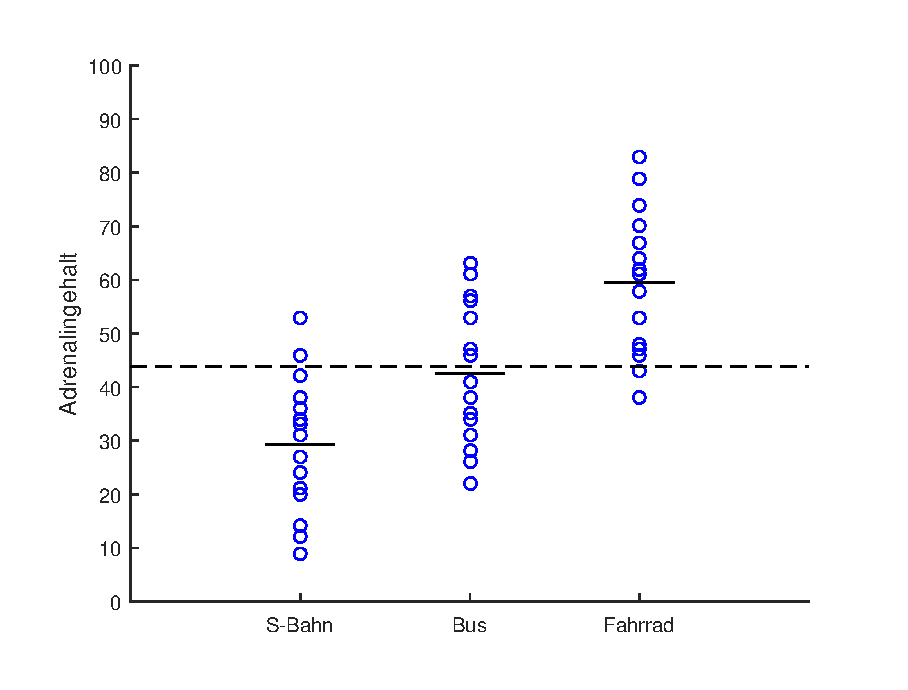
\includegraphics[width=\linewidth]{Bilder/stress}
	\end{frame}
	
	\begin{frame}{Mathematisches Modell}
		\textbf{Allgemeines Modell der einfaktoriellen Varianzanalyse} 
		\begin{center}
			\begin{tikzpicture}[thick,scale=0.8, every node/.style={scale=0.8}]
			\tikzstyle{myedgestyle} = [-triangle 60]
			
			
			\node at (-5,1.5) {$y_{k} = \mu + \alpha_k + \varepsilon_{k}$};
			\node (A1) at (-7.5,3) {Zielvariable};
			\node (A2) at (-6.4,1.8) {};
			
			\node at (-5.4,1.2)(B2) {};
			\node [align=left] (B1) at (-5.8,-0.2) {Mittelwert der\\Gesamtstichprobe};
			\node at (-4.6,1.8)(C2) {};
			\node [align=left] (C1) at (-2.8,3) {Effekt der Faktorstufe $i$\\(systematische Varianz)};
			\node at (-3.6,1.4) (D2){};
			\node [align=left] (D1) at (-0.4,1.4) {Verbleibender Fehler\\(Fehlervarianz)};
			
			
			\node at (-9.4,-2.2) {$k = 1,\dots ,K, n =1,\dots,N_k$};
			\node at (-9.6,-2)(E2) {};
			\node [align=left] (E1) at (-10,-0.8) {Anzahl der Faktorstufen des\\betrachteten Faktors};
			\node (F2) at (-7.4,-2.2) {};
			\node [align=left] (F1) at (-4,-2.4) {Stichprobenumfänge f\"ur\\die einzelnen Faktorenstufen};
	
			\draw [myedgestyle] (A1) -- (A2);
			\draw [myedgestyle] (B1) -- (B2);
			\draw [myedgestyle] (C1) -- (C2);
			\draw [myedgestyle] (D1) -- (D2);
			\draw [myedgestyle] (E1) -- (E2);
			\draw [myedgestyle] (F1) -- (F2);
			
			
			\end{tikzpicture}
		\end{center}
	\end{frame}
	
		\begin{frame}{Mathematisches Modell}
			\textbf{Allgemeines Modell der zweifaktoriellen Varianzanalyse} 
			\begin{center}
				\begin{tikzpicture}[thick,scale=0.8, every node/.style={scale=0.8}]
				\tikzstyle{myedgestyle} = [-triangle 60]
				
				
				\node at (-5,1.5) {$y_{jk} = \mu + \alpha_j  + \beta_k + (\alpha\beta)_{jk}+ \varepsilon_{jk}$};
				\node (A1) at (-9.8,2.2) {Zielvariable};
				\node (A2) at (-7.6,1.6) {};
				
				\node (B2) at (-6.5,1.2) {};
				\node [align=left] (B1) at (-7.2,-0.5) {Mittelwert der\\Gesamtstichprobe};
				\node (C2) at (-5.8,1.8) {};
				\node [align=left] (C1) at (-6,3.6) {Effekt der Faktorstufe $i$\\(systematische Varianz A)};
				\node (D2) at (-2.4,1.4) {};
				\node [align=left] (D1) at (1,1.4) {Verbleibender Fehler\\(Fehlervarianz)};
				
				\node (G2) at (-4,1.4) {};
				\node[align=left] (G1) at (-2.8,-0.6) {Interaktionseffekt zw. der Stufe $j$\\
					UVA und der Stufe $k$ UVB\\(systematische Varianz AxB)};
				
				\draw [myedgestyle] (A1) -- (A2);
				\draw [myedgestyle] (B1) -- (B2);
				\draw [myedgestyle] (C1) -- (C2);
				\draw [myedgestyle] (D1) -- (D2);
				\draw [myedgestyle] (G1) -- (G2);
				
				\end{tikzpicture}
			\end{center}
		\end{frame}
		
		\begin{frame}{Hypothesen}
			\begin{block}{einfaktoriell}
				\begin{itemize}\itemsep=2ex
					\item Nullhypothese:\\
					Alle Mittelwerte sind gleich oder alle Effekte $\alpha_k$ sind 0.\\
					Formal: $H_0: \mu_1 = \mu_2 = \dots = \mu_k$ oder $\sum\alpha_k^2=0$
					\item Alternativhypothese:\\
					Nicht alle Mittelwerte sind gleich oder mindestens ein Effekt $\alpha_i$ ist ungleich Null.\\
					Formal: $H_1: \sum(\mu_k-\mu)^2 > 0$ oder $\sum\alpha_k^2>0$
				\end{itemize}
			\end{block}
		\end{frame}
		
		\begin{frame}{Hypothesen}
			\begin{block}{zweifaktoriell}
				Für jeden Faktor wird eine Nullhypothese überprüft
				\begin{itemize}\itemsep=1ex
					\item Faktor A:\\
					Alle Zeilenmittelwerte sind gleich oder alle Effekte $\alpha_j$ sind 0.\\
					Formal: $H_0: \mu_{1\cdot} = \mu_{2\cdot} = \dots = \mu_{J\cdot}$ oder $\sum\alpha_j^2=0$
					\item Faktor B:\\
					Alle Spaltenmittelwerte sind gleich oder alle Effekte $\beta_k$ sind 0.\\
					Formal: $H_0: \mu_{\cdot1} = \mu_{\cdot2} = \dots = \mu_{\cdot K}$ oder $\sum\beta_k^2=0$
					\item Interaktion AB:\\
					Die Wirkung der einzelnen UVn auf die AV ist voneinander abhängig.\\
					Formal: $H_0: \bar{y}_{jk} = \mu_{\cdot k} + \mu_{j\cdot} - \mu + \varepsilon$
				\end{itemize}
			\end{block}
		\end{frame}
		\begin{frame}{Zweifaktorielle Varianzanalyse}
			
			\begin{table}[]
				\centering
				\resizebox{\textwidth}{!} {
				\begin{tabular}{|cc|c|c|c|c|c|}
					\hline
					\multicolumn{2}{|c|}{\multirow{2}{*}{}}        & \multicolumn{4}{c|}{UV B}                                                                                        & Zeilenmittel           \\
					\multicolumn{2}{|c|}{}                         & $B_1$                       & $B_2$                       & \dots                  & $B_K$                       & HE A                   \\ \hline
					\multirow{8}{*}{UV A} & \multirow{2}{*}{$A_1$} & \multirow{2}{*}{$\mu_{11}$} & \multirow{2}{*}{$\mu_{12}$} & \multirow{2}{*}{\dots} & \multirow{2}{*}{$\mu_{1K}$} & $\mu_{1\cdot}$         \\
					&                        &                             &                             &                        &                             & $= \mu + \alpha_1$     \\ \cline{2-7} 
					& \multirow{2}{*}{$A_2$} & \multirow{2}{*}{$\mu_{21}$} & \multirow{2}{*}{\dots}      & \multirow{2}{*}{\dots} & \multirow{2}{*}{\dots}      & $\mu_{2\cdot}$         \\
					&                        &                             &                             &                        &                             & $= \mu + \alpha_2$     \\ \cline{2-7} 
					& \multirow{2}{*}{\dots} & \multirow{2}{*}{\dots}      & \multirow{2}{*}{\dots}      & \multirow{2}{*}{\dots} & \multirow{2}{*}{\dots}      & $\mu_{j\cdot}$         \\
					&                        &                             &                             &                        &                             & $= \mu + \alpha_j$     \\ \cline{2-7} 
					& \multirow{2}{*}{$A_J$} & \multirow{2}{*}{$\mu_{J1}$} & \multirow{2}{*}{\dots}      & \multirow{2}{*}{\dots} & \multirow{2}{*}{$\mu_{JK}$} & $\mu_{J\cdot}$         \\
					&                        &                             &                             &                        &                             & $= \mu + \alpha_J$     \\ \hline
					Spalten-              & \multirow{2}{*}{HE B}  & $\mu_{\cdot1}$              & $\mu_{\cdot2}$              & $\mu_{\cdot k}$        & $\mu_{\cdot K}$             & \multirow{2}{*}{$\mu$} \\
					mittel                &                        & $= \mu + \beta_1$           & $= \mu + \beta_2$           & $= \mu + \beta_k$      & $= \mu + \beta_K$           &                        \\ \hline
				\end{tabular}
			}
			\end{table}
		\note{Frage ans Publikum: Wie sieht dreifaktoriell aus?\\
			Dreifaktoriell: "Zeilen-/ Spaltenmittel" sind dann ganze Tabellen\\
			Also immer Itteration über alle Faktorstufen aller anderer Faktoren\\
			Beispiel: Schicht in Rubixcube}
		\end{frame}
	\section{Prinzip der Varianzanalyse}
		
	\againframe{prinzipVA}
	
	\begin{frame}{Summe der Abweichungsquadrate}
		Repräsentiert die Unterschiedlichkeit der Werte der AV.
		Drei relevante Formen:
		\begin{itemize} \itemsep=2ex
			\item $SAQ_{Gesamt}$: Die Gesamtvariabilität.\\
			Formal: $SAQ_{Gesamt}= \sum(y - \bar{y})^2$
			\item $SAQ_{Effekt}$: auch $SAQ_{zwischen}$; Variabilität zwischen Bedingungen.\\
			Formal: $SAQ_{Effekt} = n_k \sum_{k=1}^{K} (\bar{y}_k - \bar{y})^2$ 
			\item $SAQ_{Fehler}$: auch $SAQ_{innerhalb}$; Variabilität innerhalb einer Bedingung.\\
			Formal: $SAQ_{Fehler} = \sum (y - \bar{y}_k)^2$ 
		\end{itemize}
		\begin{center}
			\textbf{Es gilt $\mathbf{SAQ_{Gesamt} = SAQ_{Effekt} + SAQ_{Fehler}}$}
		\end{center}
	\end{frame}
	
	\againframe{beispiel1}
		
	\begin{frame}{Freiheitsgrade (FG)}	
		
		Anzahl der frei variierbaren Werte oder auch \\
		Anzahl der in die SAQ eingehenden Werte
		\begin{itemize}
			\item $SAQ_{Gesamt}$: $N-1$
			\item $SAQ_{Effekt}$: $K-1$ \hspace{3em} K: Anzahl Faktorstufen
			\item $SAQ_{Effekt}$: $K \cdot (n-1)$
		\end{itemize}
		\textbf{Es gilt $\mathbf{FG_{Gesamt} = FG_{Effekt} + FG_{Fehler}}$}

	\end{frame}
	
	\begin{frame}{Mittlere Quadratsumme (MQ)}
		\begin{itemize}\itemsep=2ex
			\item Die mittlere Quadratsumme entspricht der Varianz
			\item $MQ_{Fehler}$: Schätzung der Populationsvarianz
			\item $MQ_{Effekt}$: Schätzung der Populationsvarianz wenn $H_0$ gilt
			\item Mittlere Quadratsummen sind \textbf{nicht} additiv
		\end{itemize}
		\begin{center}
			$MQ = \frac{SAQ}{FG}$
		\end{center}
	\end{frame}
	
	\begin{frame}{Bedeutung der MQ}
		\begin{itemize}\itemsep=2ex
			\item $MQ_{Effekt} = MQ_{Fehler}$: $H_0$ ist gültig
			\item $MQ_{Effekt} \gg MQ_{Fehler}$: $H_0$ ist ungültig, $MQ_{Effekt}$ enthält systematische Varianz
		\end{itemize}
		\begin{center}
			\textbf{Aber:} Wann ist $MQ_{Effekt}$ überzufällig größer als $MQ_{Fehler}$?
			\pause\\ \hfill\\ $\Rightarrow$ Prüfen mit F-Verteilung \vspace{2ex} \\
			$F = \frac{MQ_{Effekt}}{MQ_{Fehler}}, FG=K-1,K(n-1)$
		\end{center}
		
	\end{frame}
	
	\begin{frame}{F-Verteilung}
		Wenn $F_{empirisch} > F_{kritisch} \Rightarrow $ Ablehnung von $H_0$
		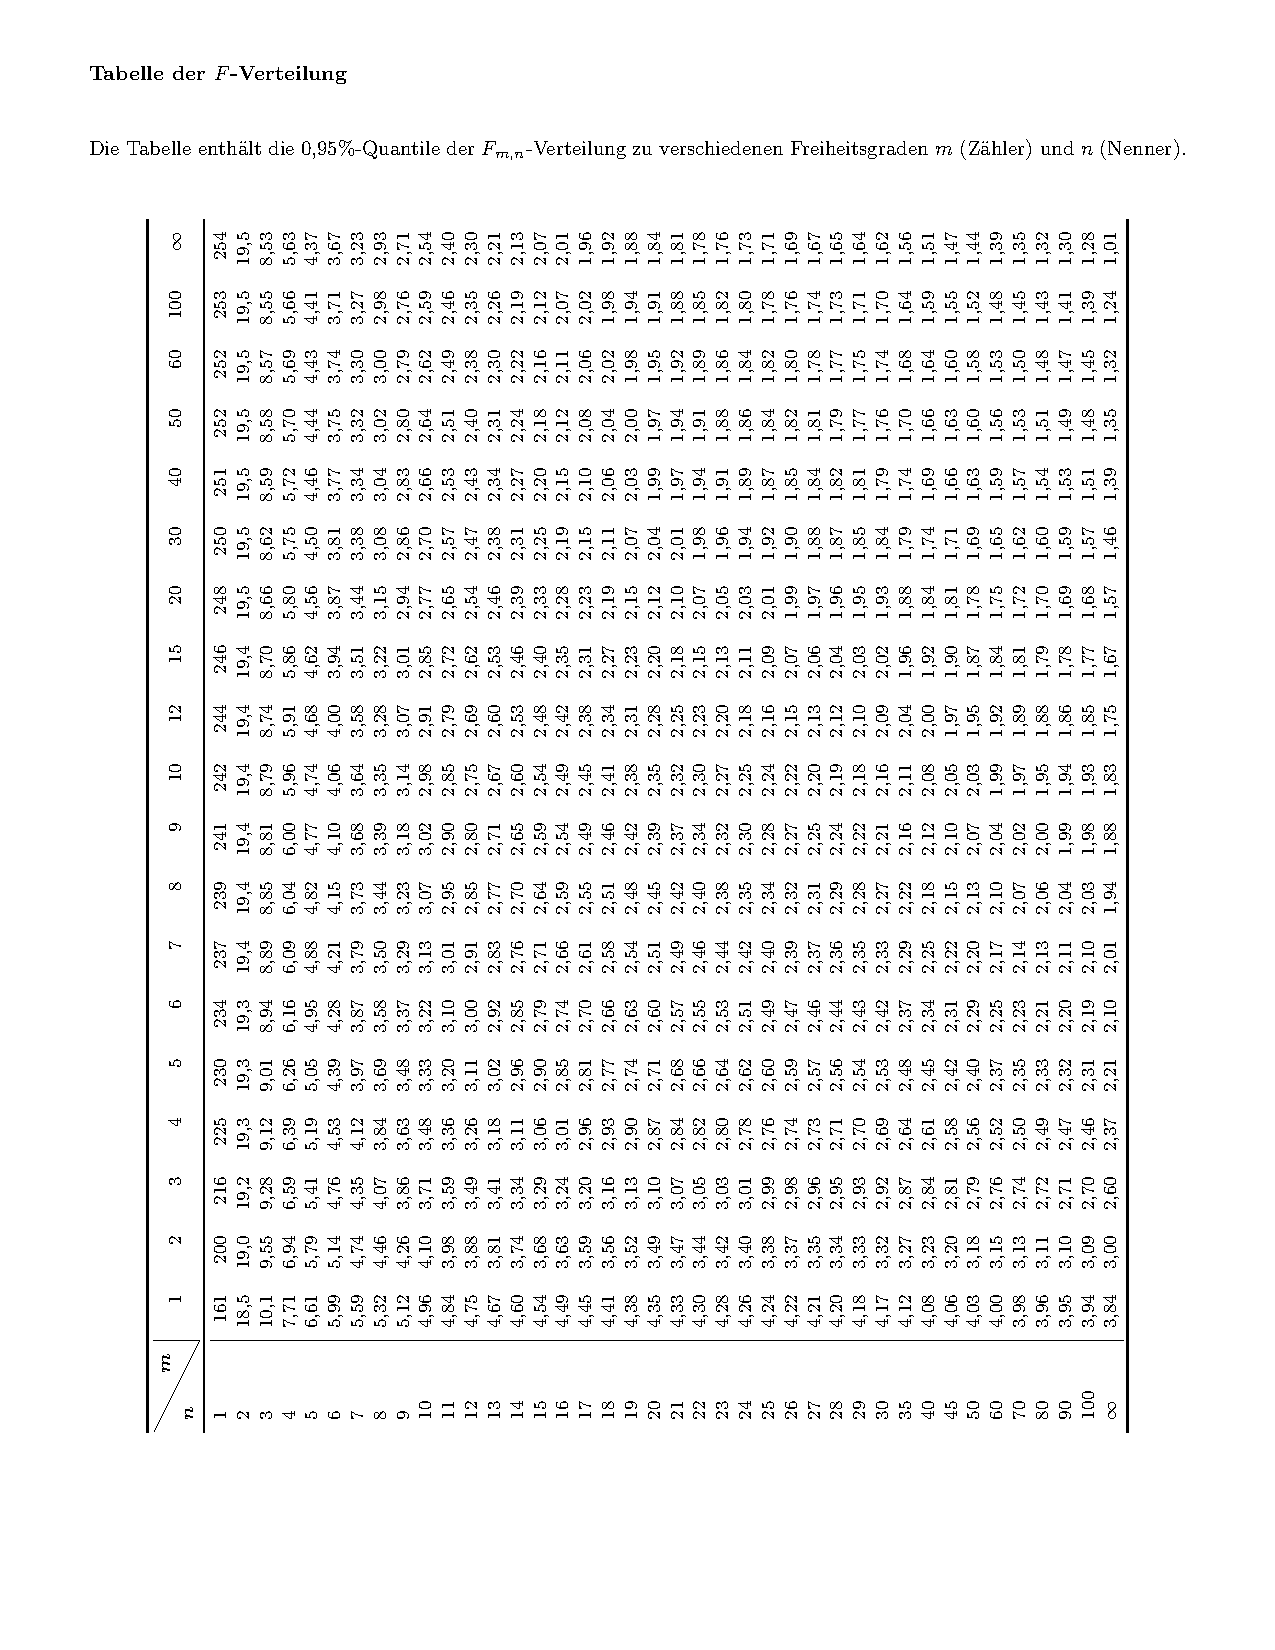
\includegraphics[trim=60 100 240 190,clip,angle=270,origin=c, width=\textwidth]{Bilder/F-verteilung}
		\let\thefootnote\relax\footnote{{\fontsize{5}{5} \selectfont \vspace{-5ex}
				Quelle: https://www.statistik.tu-dortmund.de/fileadmin/user\_upload/Lehrstuehle/Oekonometrie/Lehre/WiSo-Stat-1415/tabelleF.pdf}}
	\end{frame}
	
	\begin{frame}{F-Verteilung}
		\begin{center}
			\textbf{Was ist dieses $F$ überhaupt?}
		\end{center}
		\textbf{allgemeine Mathematiker:} \emph{$F$ ist der Quotient zweier Chi-Quadrat-Verteilter Zufallsvariablen normiert um ihre Freiheitsgrade.} \\ \vspace{0.7ex}
		\pause
		
		\textbf{Statistiker:} \emph{$F$ ist das Verhältnis der Varianzen zweier Zufallsvariablen.}\\
		\vspace{0.7ex} \pause
		\textbf{Freie Interpretation:} \emph{$F$ ist das Verhältnis zweier Stichprobenvarianzen dividiert durch ihre erwartete Varianz} \\ \vspace{0.7ex} \pause
		\begin{center}
			\textbf{Wer hat Recht? }
			\\ \vspace{0.7ex} \pause \note<.>{\alert{{\Large \textbf{Häää?!?!}} }}
			\alert{{\Large \textbf{Häää?!?!}} }
		\end{center}
	\end{frame}
	
	\begin{frame}<1-4>[label=fverteilung]{F-Verteilung}
		\begin{center}
			\textbf{Was ist dieses $F$ überhaupt?}
		
		\pause[]$F=\frac{\chi^2_m}{\chi^2_n}$\pause[3] $=\frac{MQ_{Effekt}}{MQ_{Fehler}}$\pause[4] $=\frac{\frac{s_x^2}{\sigma_x^2}}{\frac{s_y^2}{\sigma_y^2}}$\pause[5]  $=\frac{\chi^2_m}{\chi^2_n}$ 
		\end{center}
		\pause[2]~\\ \vspace{1.2ex}
		\textbf{allgemeine Mathematiker:} \emph{$F_{m,n}=\frac{\chi^2_m}{\chi^2_n}$}   
		 \pause[3] ~\\ \vspace{1.2ex}
		\textbf{Statistiker:} $F = \frac{MQ_{Effekt}}{MQ_{Fehler}}, FG=K-1,K(n-1)$ \pause[4] ~\\  \vspace{1.2ex} 
		\textbf{Freie Interpretation:} $F = \frac{\frac{s_x^2}{\sigma_x^2}}{\frac{s_y^2}{\sigma_y^2}}$ \pause[5]  $=\frac{\chi^2_m}{\chi^2_n}$ ~\\
	\end{frame}
	
	\begin{frame}{Chi-Quadrat-Verteilung}
		\begin{block}{Definition}
			Beschreibt die Verteilung der Summen von $n$ stochastisch unabhängigen quadrierten standardnormalverteilten Zufallsvariablen. \\ \vspace{2 ex}
			\textbf{Formal:} $\chi_n^2 \sim Z_1^2+ \dots + Z_n^2 $ mit $Z_k \sim \mathcal{N}(0,1)$ für $k=1, \dots , n$
			\note{$\sim$: "'ist verteilt wie"' \\Keine negativen Werte da quadrierte Summe}
		\end{block}
			\textbf{Normalverteilung zu Std.-Normalverteilung:} $Z = \frac{X-\mu}{\sigma}$ 
	\end{frame}
	
	\begin{frame}{Chi-Quadrat-Verteilung}
		Wir haben Stichprobe $X\sim \mathcal{N}(\mu,\sigma^2)$ mit Erwartungswert $\mu$ und Varianz $\sigma^2$.\\ \vspace{1ex} 
		Schätzer für Varianz der Stichprobe: $\hat{\sigma}^2 = \frac{1}{n} \sum_{i=1}^{n}(X_i-\mu)^2$ \\ \vspace{2ex}
		Dann können wir zeigen: \\
		\begin{center}
			$\frac{n\hat{\sigma}^2}{\sigma^2} = \sum_{i=1}^{n}(\frac{X_i-\mu}{\sigma})^2 =  \sum_{i=1}^{n}(Z_i) \sim \chi^2_n$
		\end{center}
		\textbf{Folgerung}\\
		Die Chi-Quadrat-Verteilung beschreibt das Verhältnis zwischen Stichproben- und Populationsvarianz in Abhängigkeit des Stichprobenumfanges $n$.
	\end{frame}
	
	\againframe<5>{fverteilung}
	
	\begin{frame}{Maß der Effektgröße}
		$\mathbf{Eta^2}$\\
		Anteil der Variation in den Daten, der durch die Variation der UV erklärt werden kann.\\
		\begin{center}
			$\eta^2 = \frac{SAQ_{Effekt}}{SAQ_{Gesamt}}$ 
		\end{center}
		\textbf{Klassifikation nach Cohen:}
		\begin{itemize}
			\item klein: 0.01
			\item mittel: 0.06
			\item groß: 0.14
		\end{itemize}
		
	\end{frame}
	
	\begin{frame}[label=VAPlan]{Varianzanalyseplan}
		Einfaktorielle Varianzanalyse\\
		\begin{table}[]
			\centering
			\resizebox{\textwidth}{!} {
			\begin{tabular}{|c|r|r|r|r|r|r|r|}
				\hline
				\multirow{2}{*}{Quelle} & \multicolumn{1}{c|}{\multirow{2}{*}{SAQ}} & \multicolumn{1}{c|}{\multirow{2}{*}{FG}} & \multicolumn{1}{c|}{\multirow{2}{*}{MQ}} & \multicolumn{1}{c|}{\multirow{2}{*}{F-Wert}} & \multicolumn{1}{c|}{F-krit}        & \multicolumn{1}{c|}{\multirow{2}{*}{Bewertung}} & \multicolumn{1}{c|}{\multirow{2}{*}{$\eta^2$}} \\
				& \multicolumn{1}{c|}{}                     & \multicolumn{1}{c|}{}                    & \multicolumn{1}{c|}{}                    & \multicolumn{1}{c|}{}                        & \multicolumn{1}{c|}{$\alpha=0.05$} & \multicolumn{1}{c|}{}                           & \multicolumn{1}{c|}{}                          \\ \hline
				Effekt                  & 22,93                                     & 2                                        & 11,46                                    & 1,22                                         & 3,89                               & n.s.                                            & 0,17                                           \\ \hline
				Fehler                  & 112,40                                    & 12                                       & 9,36                                     &                                              &                                    &                                                 &                                                \\ \hline
				Gesamt                  & 135,33                                    & 14                                       &                                          &                                              &                                    &                                                 &                                                \\ \hline
			\end{tabular}
		}
		\end{table}
		
	\end{frame}
	
	\begin{frame}{Varianzanalyseplan}
		Zweifaktorielle Varianzanalyse\\
		\begin{table}[]
			\centering
			\resizebox{\textwidth}{!} {
			\begin{tabular}{|c|r|r|r|r|r|r|r|}
				\hline
				\multirow{2}{*}{Quelle} & \multicolumn{1}{c|}{\multirow{2}{*}{SAQ}} & \multicolumn{1}{c|}{\multirow{2}{*}{FG}} & \multicolumn{1}{c|}{\multirow{2}{*}{MQ}} & \multicolumn{1}{c|}{\multirow{2}{*}{F-Wert}} & \multicolumn{1}{c|}{F-krit}        & \multicolumn{1}{c|}{\multirow{2}{*}{Bewertung}} & \multicolumn{1}{c|}{\multirow{2}{*}{$\eta^2$}} \\
				& \multicolumn{1}{c|}{}                     & \multicolumn{1}{c|}{}                    & \multicolumn{1}{c|}{}                    & \multicolumn{1}{c|}{}                        & \multicolumn{1}{c|}{$\alpha=0.05$} & \multicolumn{1}{c|}{}                           & \multicolumn{1}{c|}{}                          \\ \hline
				Haupteffekt A           & 16,054                                    & 1                                        & 16,054                                   & 2,188                                        & 4,0                                & n.s.                                            & 0,029                                          \\ \hline
				Haupteffekt B           & 34,030                                    & 2                                        & 17,015                                   & 2,319                                        & 3,15                               & n.s.                                            & 0,062                                          \\ \hline
				Interaktion AxB         & 15,528                                    & 2                                        & 7,764                                    & 1,058                                        & 3,15                               & n.s.                                            & 0,028                                          \\ \hline
				Primär                  & 65,612                                    & 5                                        & 13,122                                   & 1,789                                        & 2,37                               & n.s.                                            & 0,119                                          \\ \hline
				Fehler                  & 484,170                                   & 66                                       & 7,336                                    &                                              &                                    &                                                 &                                                \\ \hline
				Gesamt                  & 549,782                                   & 71                                       &                                          &                                              &                                    &                                                 &                                                \\ \hline
			\end{tabular}
		}
		\end{table}
	\end{frame}
	
	\section{Rechnung an Tafel}
	
	\section{Messwiederholungen}
	
	\begin{frame}{Allgemein}
		\begin{itemize}
			\item Ziel: Höhere Präzision
			\item Fehlervarianz unterteilt in interindividuelle Varianz und Restvarianz
			\item "'Normalisierung der Ausgangslage"'
		\end{itemize}
		\begin{tikzpicture}
		\draw (-0.5,0) rectangle (9.5,1.5) node[pos=.5] {Gesamt-SAQ};
		\draw  (-0.5,0) rectangle (4.5,-1.5)  node[pos=.5] {$SAQ_{Effekt}$}; 
		\draw  (4.5,0) rectangle (9.5,-1.5) node[pos=.5] {$SAQ_{Fehler}$};
		\draw[fill=black!25]  (4.5,-1.5) rectangle (7,-3) node[pos=.5][align=center] {$SAQ_{Block}$\\ \footnotesize Personen};
		\draw  (7,-1.5) rectangle (9.5,-3) node[pos=.5][align=center] {$SAQ_{Rest}$\\ \footnotesize Fehler};
		\end{tikzpicture}		
	\end{frame}
	
	\begin{frame}{Beispiel}
		Beispiel: Recallexperiment: Verschiedene Wortarten
		\begin{table}[]
			\centering
			\begin{tabular}{|l|l|l|l|}
				\hline
				\multirow{2}{*}{Vp} & \multicolumn{3}{l|}{Stufe der UV} \\
				& Substantive  & Verben & Adjektive \\ \hline
				1                   & 5            & 6      & 3         \\ \hline
				2                   & 9            & 10     & 4         \\ \hline
				3                   & 1            & 0      & 0         \\ \hline
				4                   & 4            & 2      & 2         \\ \hline
				5                   & 3            & 2      & 0         \\ \hline
			\end{tabular}
		\end{table}
		$\Rightarrow$ Unterschiede zwischen Probanden (z.B. Vp 2 und Vp 3) schlägt sich auf $SAQ_{Fehler}$ nieder.
	\end{frame}
	
	\begin{frame}{Berechnung}
		\begin{block}{Einfaktoriell}
			\begin{itemize}\itemsep=1ex
				\item $SAQ_{Block}$ bleibt unberücksichtigt
				\item $SAQ_{Block} = k \sum_{j=1}^{n}(\bar{y_j}- \bar{y})^2$ mit $k$ Messungen und $n$ VPn
				\item $SAQ_{Rest} = SAQ_{Gesamt} - SAQ_{Effekt} - SAQ_{Block}$
				\item $MQ_Rest = \frac{SAQ_{Rest}}{FG_{Rest}}$
				\item $F = \frac{MQ_{Effekt}}{MQ_{Rest}}$
			\end{itemize}
		\end{block}
	\end{frame}
	
	\begin{frame}{Varianzanalysetafel}
		\begin{block}{Einfaktorielle Varianzanalyse}
				\begin{table}[]
					\centering
					\resizebox{\textwidth}{!} {
					\begin{tabular}{|l|r|r|r|r|r|r|r|}
						\hline
						Quelle  & \multicolumn{1}{l|}{SAQ} & \multicolumn{1}{l|}{FG} & \multicolumn{1}{l|}{MQ} & \multicolumn{1}{l|}{F-Wert} & \multicolumn{1}{l|}{F-krit} & \multicolumn{1}{l|}{Bewertung} & \multicolumn{1}{l|}{$\eta^2$} \\ \hline
						Effekt  & 22,933                   & 2                       & 11,467                  & 7,398                       & 4,459                       & s.                              & 0,169                         \\ \hline
						Block   & 100,000                  & 4                       & 25,000                  & 16,123                      & 3,838                       &                                & 0,739                         \\ \hline
						Fehler  & 12,400                   & 8                       & 1,555                   &                             &                             &                                &                               \\ \hline
						Varianz & 135,333                  & 14                      &                         &                             &                             &                                &                               \\ \hline
					\end{tabular}
				}
				\end{table}
		\end{block}
	\end{frame}
	
	\againframe{VAPlan}
	
	\begin{frame}{Berechnung}
		\begin{block}{Zweifaktorielle Varianzanalyse}
			\begin{center}
				\begin{tikzpicture}[thick,scale=0.55, every node/.style={scale=0.55}]
				\draw (-5.5,0) rectangle (14.5,1.5) node[pos=.5] {Gesamt-SAQ};
				\draw  (-5.5,0) rectangle (4.5,-1.5)  node[pos=.5] {$SAQ_{Effekt}$}; 
				\draw  (4.5,0) rectangle (14.5,-1.5) node[pos=.5] {$SAQ_{Fehler}$};
				\draw  (-5.5,-1.5) rectangle (-2.17,-3)  node[pos=.5] {$SAQ_{EffektA}$}; 
				\draw  (-2.17,-1.5) rectangle (1.16,-3)  node[pos=.5] {$SAQ_{EffektB}$}; 
				\draw  (1.16,-1.5) rectangle (4.5,-3)  node[pos=.5] {$SAQ_{EffektAxB}$}; 
				
				\draw[fill=black!25]  (4.5,-1.5) rectangle (7,-3) node[pos=.5][align=center] {$SAQ_{Block}$\\ \footnotesize Personen};
				\draw  (7,-1.5) rectangle (9.5,-3) node[pos=.5][align=center] {$SAQ_{RestA}$\\ \footnotesize Fehler A};
				\draw  (9.5,-1.5) rectangle (12,-3) node[pos=.5][align=center] {$SAQ_{RestB}$\\ \footnotesize Fehler B};
				\draw  (12,-1.5) rectangle (14.5,-3) node[pos=.5][align=center] {$SAQ_{RestAxB}$\\ \footnotesize Fehler AxB};
				\end{tikzpicture}
			\end{center}
		\end{block}
	\end{frame}
	
	%----------------------------------------------------------------------------Henri-Robert-Linie---------------------------
	
	\section{Interaktion}
	
	\begin{frame}{Arten der Interaktion}
	Interaktion findet immer zwischen (mindestens) zwei unterschiedlichen UV statt
		\begin{itemize}
			\item Nullinteraktion
			\item ordinale Interaktion
			\item disordinale Interaktion
			\item semidisordinale Interaktion
		\end{itemize}
		\note{
			Interaktion findet immer zwischen (mindestens) zwei unterschiedlichen unabhängigen Variablen statt\\
			4 verschiedene Arten möglicher Interaktion\\
			\begin{itemize}
				\item Nullinteraktion
				\item ordinale Interaktion
				\item disordinale Interaktion
				\item semidisordinale Interaktion
			\end{itemize}
		}
	\end{frame}
	
	
	\begin{frame}{Nullinteraktion}
		\begin{itemize}
			\item keine Interaktion
			\item Auswirkungen einer UV sind auf allen Stufen der anderen UV gleich
			\item UVs wirken unabhängig voneinander auf die AV
			\item Die Kenntnis der Wirkung beider UVs reicht aus, um den Mittelwert jeder Zelle voraussagen zu können
			\item im Liniendiagramm: parallel
		\end{itemize}
		\note{
			\begin{itemize}
				\item keine Interaktion
				\item Auswirkungen einer UV sind auf allen Stufen der anderen UV gleich
				\item UVs wirken unabhängig voneinander auf die AV
				\item Die Kenntnis der Wirkung beider UVs reicht aus, um den Mittelwert jeder Zelle voraussagen zu können \textbf{4. Zellen sind dabei ``Untergruppen''}
				\item im Liniendiagramm: parallel
			\end{itemize}
			}
	\end{frame}
	
	\begin{frame}{Nullinteraktion - Diagramm}
		\begin{figure}
			\centering
			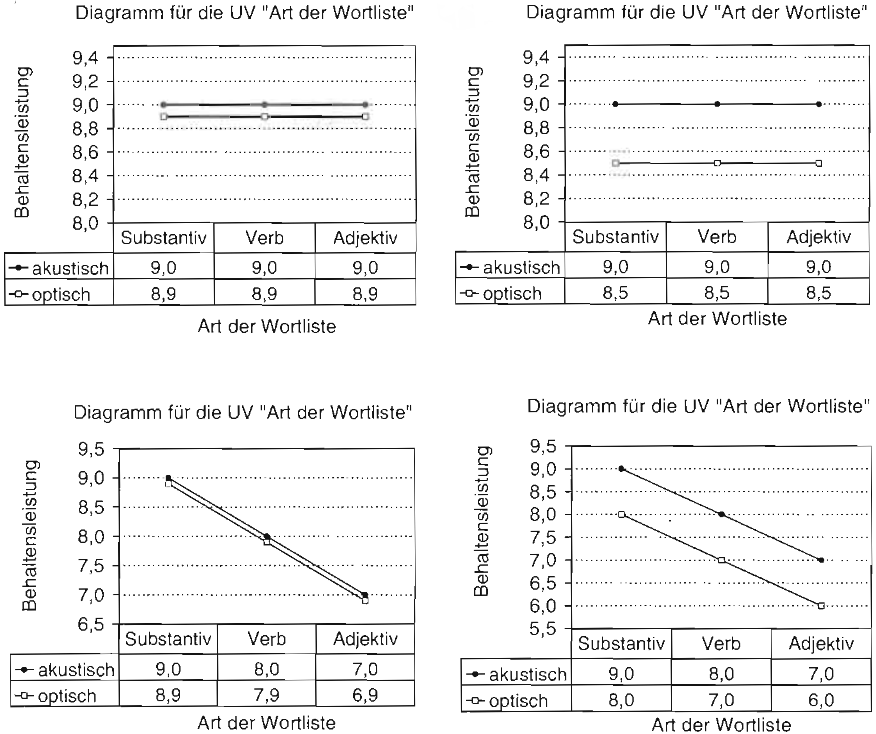
\includegraphics[width=0.8\textwidth]{Bilder/NullI.png}
		\end{figure}
		
		 \note{
		 	\footnotesize
		 Auf die unterschiedlichen Daten achten\\
		 \begin{itemize}
			\item oben links: Unterschiedliche Ausprägungen der Faktorstufe haben gleiche Werte; keine Signifikanz\\ 
			\item oben rechts UV ``Präsentationsart'' unterscheidet sich von UV ``Wortart'' aber keine Abhängigkeit voneinander; keine Signifikanz bei der Wortart
			\item unten links Umgekehrter Fall zu oben rechts; keine Signifikanz bei der Präsentationsart
			\item unten rechts oben rechts und unten links kombiniert. Trotzdem parallel $\rightarrow$ keine Interaktion. Betrachtung der Daten legt ebenfalls nahe, dass keine Abhängigkeit besteht; Signifikanz bei beiden UV
		\end{itemize}
		Bild mit vertauschten Achsen an die Tafel malen. Nachfragen, ob jemand Liniendiagramme noch nicht verstanden hat
		 }
	\end{frame}
	
	\begin{frame}{ordinale Interaktion}
		\begin{itemize}
			\item liegt vor, wenn sich eine UV auf verschiedenen Stufen der anderen UV unterschiedlich stark auswirkt
			\item Liniendiagramm: Linien nicht parallel, kreuzen sich aber auch nicht (irrelevant, welche UV wie aufgetragen wird)
			%\item Linien zeigen in dieselbe Richtung, genauer: Alle nach oben/ unten
		\end{itemize}
		 \note{
		 	Umgangssprachlich: gegenseitig verstärkende Interaktion
		 	
		 	\begin{itemize}
		 		\item liegt vor, wenn sich eine UV auf verschiedenen Stufen der anderen UV unterschiedlich stark auswirkt
		 		\item Liniendiagramm: Linien nicht parallel, kreuzen sich aber auch nicht (irrelevant, welche UV wie aufgetragen wird)
		 		%\item Linien zeigen in dieselbe Richtung, genauer: Alle nach oben/ unten
		 	\end{itemize}
		 	}
	\end{frame}
	
	\begin{frame}{ordinale Interaktion - Diagramm}
		\begin{figure}
			\centering
			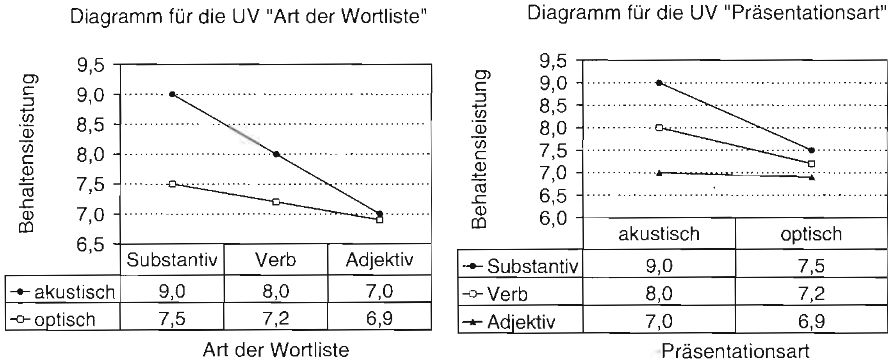
\includegraphics[width=1.0\textwidth]{Bilder/ordinaleI.png}
		\end{figure}
		\note{
			tatsächlich sind diese Diagramme eher unintuitiv, weil beide UV keiner ``echten Metrik'' folgen.\\
			Besseres Beispiel: Wir erheben die Größe von Personen anhand der Größe ihrer Eltern (UV1) und Kinder (UV2)\\
			Siehe Blatt.
		}
	\end{frame}
	
	\begin{frame}{ordinale Interaktion - Interpretation}
		\begin{itemize}
			\item Interpretation sinnvoll und eindeutig
			\item in unserem Beispiel: akustische Präsentation ist besser als optische und Substantive können besser behalten werden als Adjektive
		\end{itemize}
		\note{
			\begin{itemize}
				\item Interpretation sinnvoll und eindeutig \textbf{\\wir sehen, dass die UV sich zwar beeinflussen und gegenseitig verstärken, können aber trotzdem Aussagen über das Verhalten machen}
				\item in unserem Beispiel: akustische Präsentation ist besser als optische und Substantive können besser behalten werden als Adjektive
			\end{itemize}
			}
	\end{frame}
	
	\begin{frame}{disordinale Interaktion}
		\begin{itemize}
			\item liegt vor, wenn sich die Rangfolge der Werte einer UV auf den verschiedenen Stufen der anderen UV umkehrt
			\item Liniendiagramm: Kreuzen der Linien (irrelevant, welche UV wie aufgetragen wird)
		\end{itemize}
		\note{
			\begin{itemize}
				\item liegt vor, wenn sich die Rangfolge der Werte einer UV auf den verschiedenen Stufen der anderen UV umkehrt 
				\item Liniendiagramm: Kreuzen der Linien (irrelevant, welche UV wie aufgetragen wird)
			\end{itemize}
			}
	\end{frame}
	
	\begin{frame}{disordinale Interaktion - Diagramm}
		\begin{figure}
			\centering
			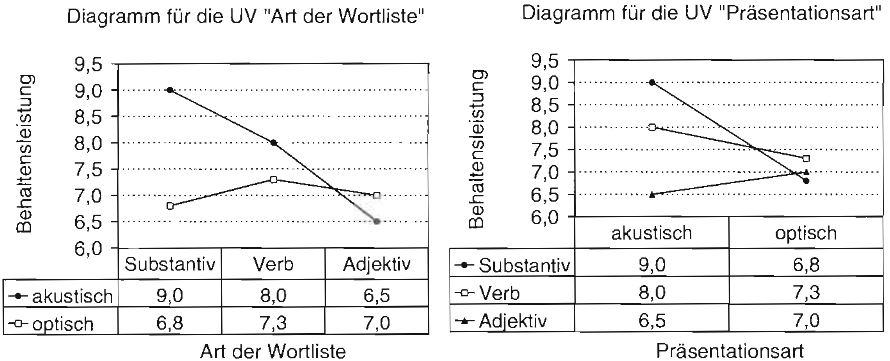
\includegraphics[width=1.0\textwidth]{Bilder/disordinaleI.png}
		\end{figure}
		\note{
		links: \\
		rechts:		
		}
	\end{frame}
	
	\begin{frame}{disordinale Interaktion - Interpretation}
		\begin{itemize}
			\item evtl. vorliegende Haupteffekte können nicht sinnvoll interpretiert werden
			\item in unserem Beispiel: Aussagen über Präsentation und Wortart sinnlos
		\end{itemize}
		\note{
			\begin{itemize}
				\item evtl. vorliegende Haupteffekte können nicht sinnvoll interpretiert werden
				\item in unserem Beispiel: Aussagen über Präsentation und Wortart sinnlos
			\end{itemize}
			}
			\note{Als nächstes kommen wir zur semidisordinalen Interaktion. Frage ans Publikum: Wir kennen jetzt ordinale und diso I, was könnte semidis sein? Vor Hintergrund des Kreuzens der Achsen}
	\end{frame}
	
	\begin{frame}{semidisordinale Interaktion} 
		\begin{itemize}
			\item auch bekannt als hybride Interaktion
			\item liegt vor, wenn für eine UV eine ordinale Interaktion vorliegt, für die andere jedoch eine disordinale Interaktion
			\item Liniendiagramm: Sowohl Kreuzen als auch nicht Kreuzen, je nachdem, welche UV wie aufgetragen wird
		\end{itemize}
		\note{
			\begin{itemize}
				\item auch bekannt als hybride Interaktion
				\item liegt vor, wenn für eine UV eine ordinale Interaktion vorliegt, für die andere jedoch eine disordinale Interaktion
				\item Liniendiagramm: Sowohl Kreuzen als auch nicht Kreuzen, je nachdem, welche UV wie aufgetragen wird
			\end{itemize}
			}
	\end{frame}
	
	\begin{frame}{semidisordinale Interaktion - Diagramm}
		\begin{figure}
			\centering
			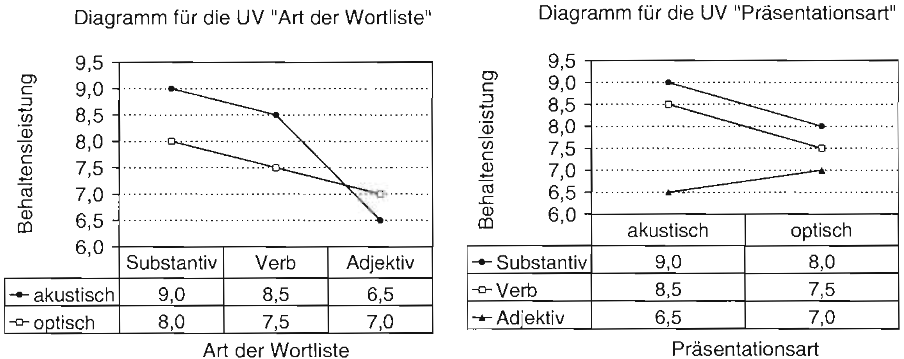
\includegraphics[width=1.0\textwidth]{Bilder/semidisordinaleI.png}
		\end{figure}
		\note{
		links: \\
		rechts:		
		}
	\end{frame}
	
	\begin{frame}{semidisordinale Interaktion - Interpretation}
		\begin{itemize}
			\item Interpretation für den ordinalen Faktor sinnvoll
			\item in unserem Beispiel: Substantive werden besser behalten als Adjektive
		\end{itemize}
		\alert{Aussage über die Präsentationsart?}
		\pause \\
		Kann nicht getroffen werden
		\note{
			\begin{itemize}
				\item Interpretation für den ordinalen Faktor sinnvoll
				\item in unserem Beispiel: Substantive werden besser behalten als Adjektive
			\end{itemize}
			\alert{Aussage über die Präsentationsart?}\\
			Kann nicht getroffen werden
			}
	\end{frame}
	
	\begin{frame}{Alternativdarstellung}
		\note{
			Unterschied zwischen der ursprünglichen und alternativen darstellung:\\
			ursprünglich: Kreuzen der Linien essentiell für disordinale Interaktion\\
			alternativ: (Aus-)Richtung der Linien essentiell, Überschneidung kann bei Disordi I vorkommen, muss aber nicht\\
			
		}
		Experiment
		\begin{itemize}
			\item Gesucht: Ursachen für Aggression
			\item Frust wird induziert, indem Probanden ein unlösbares Puzzle vorgelegt wird
			\item Kontrollgruppe mit lösbarem Puzzle
			\item als UV kommt die Raumtemperatur hinzu (20$^{\circ}$ bzw. 30$^{\circ}$)
		\end{itemize}
		Prinzip jetzt: Richtung der Linien
	\end{frame}
	
	\begin{frame}{Ordinale Interaktion alternativ}
		\begin{figure}
			\centering
			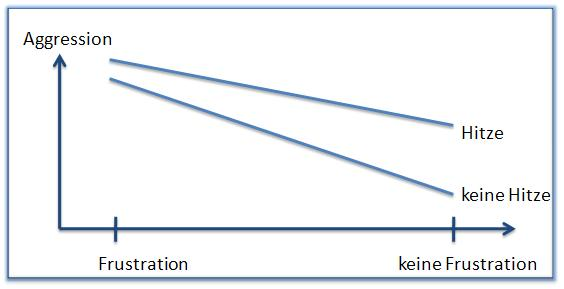
\includegraphics[width=0.6\textwidth]{Bilder/OrdinaleInteraktion1.jpg}
		\end{figure}
		\begin{figure}
			\centering
			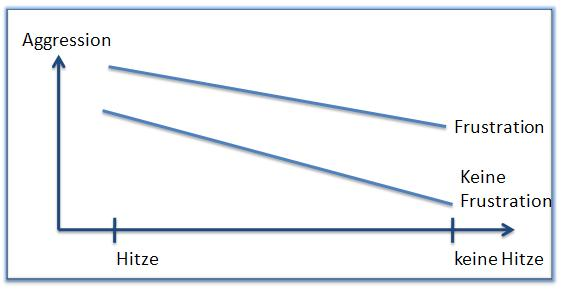
\includegraphics[width=0.6\textwidth]{Bilder/OrdinaleInteraktion2.jpg}
		\end{figure}
		\note{
			Bei der ordinalen Interaktion wird unsere Regel (Nicht-Kreuzen) erweitert\\
			Zusätzlich müssen sich beide Linien in dieselbe Richtung bewegen, z.b. sinken\\
			In diesem Beispiel: Der Wert von sowohl Hitze als auch keine Hitze muss von Frustration zu keine Frustration sinken\\
			Was sehen wir hier?\\
			Beide Achsendarstellungen der Versuchsergebnisse.\\
			Tritt auf bei ``spitzem Trichter''
			}
	\end{frame}
	
	
	\begin{frame}{Disordinale Interaktion alternativ}
		\begin{figure}
			\centering
			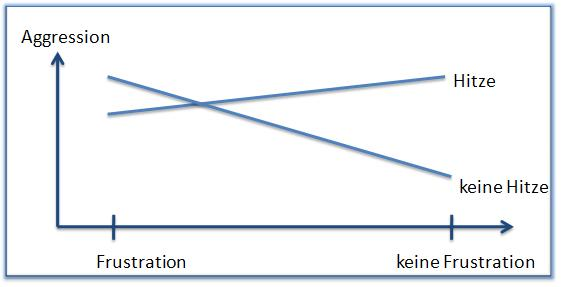
\includegraphics[width=0.6\textwidth]{Bilder/DisordinaleInteraktion1.jpg}
		\end{figure}
		\begin{figure}
			\centering
			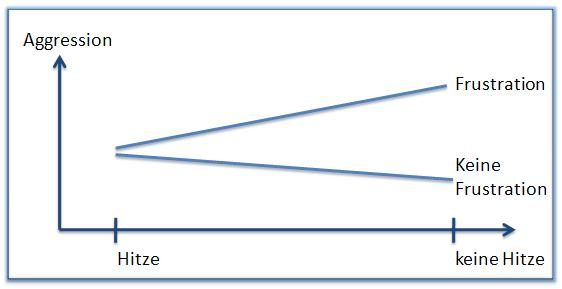
\includegraphics[width=0.6\textwidth]{Bilder/DisordinaleInteraktion2.jpg}
		\end{figure}
		\note{
			tritt auf, wenn Richtung unterschiedlich und Kreuzen auftritt\\
			kann auftreten bei ``stumpfem Trichter''
		}
	\end{frame}
	
	
	\begin{frame}{Semidisordinale Interaktion alternativ}
		\begin{figure}
			\centering
			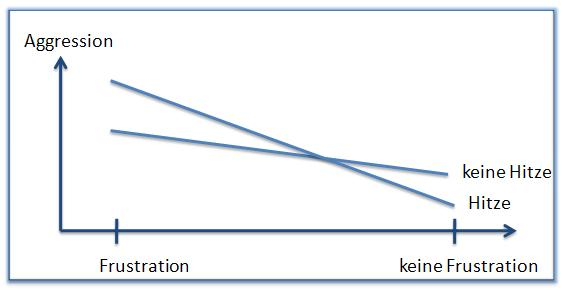
\includegraphics[width=0.6\textwidth]{Bilder/HybrideInteraktion1.jpg}
		\end{figure}
		\begin{figure}
			\centering
			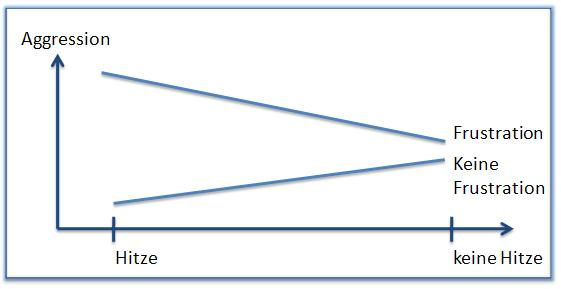
\includegraphics[width=0.6\textwidth]{Bilder/HybrideInteraktion2.jpg}
		\end{figure}
		\note{
			Tritt auf, wenn Richtung zwar gleich aber trotzdem Kreuzen auftritt\\
			Alternativ: ``Großer Trichter''
			}
	\end{frame}
	
	\begin{frame}{Interaktion alternativ - Zusammenfassung}
		\begin{itemize}
			\item Beide Linien zeigen in die selbe Richtung, ``spitzer Trichter''\\
			$\rightarrow$ ordinale Interaktion
			\item Kreuzen wegen unterschiedlicher Richtungen, ``stumpfer Trichter''\\
			$\rightarrow$ disordinale Interaktion
			\item Kreuzen trotz gleicher Richtungen, ``stumpfer Trichter''\\
			$\rightarrow$ semidisordinale Interaktion
		\end{itemize}
	\end{frame}
	
	\section{Anwendungsvoraussetzungen der Varianzanalyse}
	
	\begin{frame}{Allgemeine Voraussetzungen - Zufallsstichproben}
		\note{Zufallsstichprobe aus der Population werden in der Psychologie kaum verwendet $\rightarrow$ was bedeutet das für die Relevanz?\\}
		\begin{itemize}
			\item Die Qualität der Stichprobe ist wichtig für die Konstruktion der Stichprobenkennwerteverteilung \note{1. Stichprobenkennwerteverteilung geht von Zufallsstichprobe aus\\} \\
			 $\rightarrow$ bildet Grundlage für die Signifikanzentscheidung
			\item Falls die Stichprobe nichtzufällig gezogen ist, konstruiert man eine hypothetische Grundgesamtheit \note{2. d.h. wir tuen einfach mal so, als wäre unsere Stichprobe repräsentativ\\}
			\item für diese gilt dann die entsprechende Stichprobenkennwerteverteilung, damit können wir unser Ergebniss gegen eine Zufallserklärung absichern\note{3. falls Signifikanz vorliegt\\}
			\note{Mal nen Bild dazu an die Tafel, Spuckspasti/ Anekdote zu Nutzerstudien/ }
		\end{itemize}
		\note{Diskussionsrunde: Welchen Wert haben die an Universitäten gefundenen Ergebnisse im Hinblick auf die Zufälligkeit der Stichprobe? Zitat: ``Im übrigen zeigt gerade die psychologische Forschung, dass es offensichtlich möglich ist, auch mithilfe nichtzufälliger Stichproben zu neuen Erkenntnissen zu gelangen, da praktisch nie mit echten Zufallsstichproben gearbeitet wird''}
	\end{frame}
	
	\begin{frame}{Allgemeine Voraussetzungen - Unabhängigkeit der Messungen}
		\begin{itemize}
			\item Der Einfluss von Störvariablen für jede Messung muss unabhängig sein vom Einfluss der Störvariablen jeder anderen Messung
			\item Das gilt sowohl innerhalb der, als auch zwischen den Stichproben
			\item d.h. insbesondere, dass es keine Subgruppen innerhalb der Stichproben geben darf
		\end{itemize}
		\note{
			\footnotesize
			Beispiel Hausaufgaben: Versuch, Ziel: beste Art der Hausaufgaben-Erteilung: kurzfristig (zb. jeden Tag die für den nächsten Tag) oder langfristig (am Ende des Monats müssen eine bestimmte Menge an Aufgaben erledigt sein, freie Zeiteinteilung)\\ Stichprobe aus zwei Klassen, die jeweils mit einer der Arten vertraut sind\\ Gemeinsame Vorerfahrung sorgt für abhängige Störvariablen\\
			Anderes Beispiel: Familienmitglieder in einer Studie, bei der Inividualdaten aufgenommen werden $\rightarrow$ Sozialer Background nicht unabhängig voneinander
			\begin{itemize}
				\item Der Einfluss von Störvariablen für jede Messung muss unabhängig sein vom Einfluss der Störvariablen jeder anderen Messung
				\item Das gilt sowohl innerhalb der, als auch zwischen den Stichproben
				\item d.h. insbesondere, dass es keine Subgruppen innerhalb der Stichproben geben darf
			\end{itemize}
			}
	\end{frame}
	
	\begin{frame}{Skalenniveau}
		\begin{itemize}
			\item Varianzanalyse macht nur Aussagen über Mittelwerte\\
			$\rightarrow$ sollte nur auf Daten angewendet werden, bei denen eine Aussage über Mittelwerte sinnvoll ist
			\item d.h. die erhobenen Daten sollten mindestens einer Metrik unterliegen
			\item \alert{allerdings:} Manchmal lässt sich aus einer sinnvollen Interpretation auch auf eine sinnvolle Anwendung ``Rückschließen''\\
			$\rightarrow$ bspw. Schulnoten
		\end{itemize}
		\note{
			\begin{itemize}
				\footnotesize
				\item Varianzanalyse macht nur Aussagen über Mittelwerte
				$\rightarrow$ sollte nur auf Daten angewendet werden, bei denen eine Aussage über Mittelwerte sinnvoll ist
				\item d.h. die erhobenen Daten sollten mindestens einer Metrik unterliegen
				\item \alert{allerdings:} Manchmal lässt sich aus einer sinnvollen Interpretation auch auf eine sinnvolle Anwendung ``Rückschließen'' \textbf{hier heiligt der swag die Mittel roflcopter}
				$\rightarrow$ bspw. Schulnoten\textbf{Schulnoten: Ist 1 doppelt so gut wie 2? 4x so gut wie 4? Noten in Prozent angeben $\rightarrow$ beim Programmieren: Erste 80\% der Anforderungen brauchen 20\% der Zeit, die nächsten 20\% 80\% der Zeit}
				\textbf{anmerken, dass für die VA die ursprüngliche Population natürlich auch normalverteilt sein muss, bei anderen Verteilungen macht die VA keinen Sinn}
			\end{itemize}
			}
	\end{frame}
	
	\section{Versuch}
	\note{
		Ablauf:\\
		\begin{itemize}
			\footnotesize
			\item Leute sollen auf Zettel schreiben
			\item Wir zeigen zuerst eine Folie mit 30 Wörtern, je 10 Substantive, Verben, Adjektive
			\item für 60 Sekunden sollen die Wörter gelernt werden
			\item danach 60 Sekunden, um die Wörter aufzuschreiben
			\item kurze Pause, darin den weiteren Ablauf erklären
			\item danach soll der Zettel gedreht werden, damit die bereits geschriebenen Wörter nicht einfach copy-pasted werden
			\item eine weitere Runde lernen und aufschreiben
			\item dann die Lösung, aufgeteilt nach Substantive, Verb, Adjektiv an die Tafel werfen. dann Analyse
		\end{itemize}
		}
	
	\begin{frame}{Wörter}
		\begin{table}[]
			\centering
			%\caption{My caption}
			\label{my-label}
			\begin{tabular}{llllll}
				Schuh      & bunt     & anfeuern & Haus     & fleißig  & reisen  \\
				schreien   & Zug      & lustig   & reden    & Hund     & ulkig   \\
				groß       & wissen   & Band     & fröhlich & ausgeben & Erfolg  \\
				Eis        & schlecht & erfinden & Brille   & müde     & laufen  \\
				bestätigen & Bild     & lebhaft  & fluten   & Enkel    & schnell
			\end{tabular}
		\end{table}
		\note{
			Ablauf:\\
			\begin{itemize}
				\footnotesize
				\item Leute sollen auf Zettel schreiben
				\item Wir zeigen zuerst eine Folie mit 30 Wörtern, je 10 Substantive, Verben, Adjektive
				\item für 60 Sekunden sollen die Wörter gelernt werden
				\item danach 60 Sekunden, um die Wörter aufzuschreiben
				\item kurze Pause, darin den weiteren Ablauf erklären
				\item danach soll der Zettel gedreht werden, damit die bereits geschriebenen Wörter nicht einfach copy-pasted werden
				\item eine weitere Runde lernen und aufschreiben
				\item dann die Lösung, aufgeteilt nach Substantive, Verb, Adjektiv an die Tafel werfen. dann Analyse
			\end{itemize}
		}
	\end{frame}
	
	\begin{frame}{Auflösung}
		\begin{table}[]
			\centering
			\begin{tabular}{ll|ll|ll}
				\multicolumn{2}{c|}{\textbf{Subjektive}} & \multicolumn{2}{c|}{\textbf{Verben}} & \multicolumn{2}{c}{\textbf{Adjektive}} \\ \hline
				Schuh & Haus & schreien & reden & groß & fröhlich \\
				Eis & Brille & bestätigen & fluten & bunt & fleißig \\
				Zug & Hund & wissen & ausgeben & schlecht & müde \\
				Bild & Enkel & anfeuern & reisen & lustig & ulkig \\
				Band & Erfolg & erfinden & laufen & lebhaft & schnell
			\end{tabular}
		\end{table}
		\note{
			Ablauf:\\
			\begin{itemize}
				\footnotesize
				\item Leute sollen auf Zettel schreiben
				\item Wir zeigen zuerst eine Folie mit 30 Wörtern, je 10 Substantive, Verben, Adjektive
				\item für 60 Sekunden sollen die Wörter gelernt werden
				\item danach 60 Sekunden, um die Wörter aufzuschreiben
				\item kurze Pause, darin den weiteren Ablauf erklären
				\item danach soll der Zettel gedreht werden, damit die bereits geschriebenen Wörter nicht einfach copy-pasted werden
				\item eine weitere Runde lernen und aufschreiben
				\item dann die Lösung, aufgeteilt nach Substantive, Verb, Adjektiv an die Tafel werfen. dann Analyse
			\end{itemize}
		}
	\end{frame}
	
\end{document}

	\begin{frame}{Haupteffekte}
		Haupteffekte vs einfache Haupteffekte
		\begin{itemize}
			\item Haupteffekte = Wirkung einer UV über alle Stufen der anderen UV
			\item einfache Haupteffekte beziehen sich nur auf \textbf{eine} Stufe der anderen UV
		\end{itemize}
	\end{frame}
	
	%\section{Rechnung an Tafel}
	
	%---------------------------------- Ab hier Beispiele für Folien
	
	
	